%% talk1.tex
%% Copyright 2022 Tom M. Ragonneau
%
% This work may be distributed and/or modified under the
% conditions of the LaTeX Project Public License, either version 1.3
% of this license or (at your option) any later version.
% The latest version of this license is in
%   http://www.latex-project.org/lppl.txt
% and version 1.3 or later is part of all distributions of LaTeX
% version 2005/12/01 or later.
%
% This work has the LPPL maintenance status `maintained'.
%
% The Current Maintainer of this work is Tom M. Ragonneau.
\documentclass{polyu-presentation}
\usepackage[final]{microtype}

% List of hyphenation exceptions for US English
% Source: https://ctan.org/tex-archive/info/digests/tugboat/hyphenex
\input{ushyphex}

% Bibliographical resources
\addbibresource{ragonneau-bib/strings.bib}
\addbibresource{ragonneau-bib/optim.bib}

% Dedicated mathematical macros
\usepackage{ifthen}
\newcommand{\obj}{f}
\newcommand{\objm}[1][]{\hat{f}\ifthenelse{\equal{#1}{}}{}{^{#1}}}
\newcommand{\xpt}[1][]{\mathcal{Y}\ifthenelse{\equal{#1}{}}{}{^{#1}}}

% If-Then-Else function for pgfplots
\pgfmathdeclarefunction{ifthenelsefpu}{3}{\pgfmathparse{#1*#2 + !#1*#3}}

\title{Model-Based DFO Methods and Software}
\subtitle{Talk no.\ 2 \textemdash\ Interpolation models}
\author[Tom M. Ragonneau]{\texorpdfstring{
    Tom M. Ragonneau\\ 
    \footnotesize Co-supervised by Dr.\ Zaikun Zhang and by Prof.\ Xiaojun Chen
}{Tom M. Ragonneau}}
\institute[PolyU AMA]{
    Department of Applied Mathematics\\
    The Hong Kong Polytechnic University
}
\date{September 26, 2022}
\titlegraphic{}

\begin{document}

\begin{frame}
	\titlepage
\end{frame}

\begin{frame}
    \frametitle{Table of contents}
	\tableofcontents[hideallsubsections]
\end{frame}

\section{Elementary concepts of multivariate interpolation}

\begin{frame}
    \frametitle{Interpolation models for DFO}
    
    A polynomial~$\objm$ \alert{interpolates}~$\obj$ on~$\xpt \subseteq \R^n$ if
    \begin{equation*}
        \objm(y) = \obj(y), \quad \text{for~$y \in \xpt$.}
    \end{equation*}

    \begin{block}{}
        The \alert{dimension} of the space of polynomials on~$\R^n$ of degree at most~$k$ is
        \begin{equation*}
            \binom{n + k}{n} = \frac{1}{k!} \prod_{i = 1}^k (n + i) \ge \frac{n^k}{k!}.
        \end{equation*}

        Why?
        For the terms~$x_1^{i_1} x_2^{i_2} \dots x_n^{i_n}$, we \alert{count} the number of~$(i_1, i_2, \dots, i_n)$ with nonnegative entries and~$i_1 + i_2 + \dots + i_n \le k$.
        With~$k$ stars and~$n$ bars:

        \begin{center}
            \tikzstyle{thmstars}=[star,star points=5,star point ratio=2.25,draw,thick,inner sep=2pt]
            \begin{tikzpicture}
                \node[thmstars] at (0,0) {};
                \node[thmstars] at (1,0) {};
                \node[thmstars] at (2,0) {};
                \node[thmstars] at (3,0) {};
                \node at (4,0) {$\cdots$};
                \node[thmstars] at (5,0) {};
                \node[thmstars] at (6,0) {};

                \draw[thick] (-0.5,-0.25) -- (-0.5,0.25);
                \draw[thick] (0.4,-0.25) -- (0.4,0.25);
                \draw[thick] (0.6,-0.25) -- (0.6,0.25);
                \draw[thick] (2.5,-0.25) -- (2.5,0.25);
                \draw[thick] (5.5,-0.25) -- (5.5,0.25);
            \end{tikzpicture}
        \end{center}

        Here,~$i_1 = 0$,~$i_2 = 1$,~$i_3 = 0$,~$i_4 = 2$, etc.
        There are~$\binom{n + k}{k}$ \alert{combinations}.
    \end{block}
\end{frame}

\begin{frame}
    \frametitle{Quadratic interpolants}

    We focus on the \alert{quadratic} interpolants
    \begin{equation*}
        \objm(x) = \textcolor{OliveGreen}{c} + \textcolor{BurntOrange}{g}^{\T} x + \frac{1}{2} x^{\T} \textcolor{Maroon}{B} x.
    \end{equation*}

    \begin{block}{Poisedness~{\parencite[Def.~3.1]{Conn_Scheinberg_Vicente_2009b}}}
        The interpolation set~$\xpt \subseteq \R^n$ is \alert{poised} if for all~$\obj$ there exists a \alert{unique} quadratic interpolant~$\objm$ such that
        \begin{equation*}
            \objm(y) = \obj(y), \quad \text{for~$y \in \xpt$.}
        \end{equation*}
    \end{block}

    \medskip

    If~$\xpt$ is poised, then
    \begin{equation*}
        \card \xpt = \frac{1}{2} (n + 1) (n + 2) = \textcolor{OliveGreen}{1} + \textcolor{BurntOrange}{n} + \textcolor{Maroon}{\frac{n (n + 1)}{2}}.
    \end{equation*}
\end{frame}

\begin{frame}
    \frametitle{A basis of quadratic polynomials}

    Let~$\xpt = \set{y^1, y^2, \dots, y^m}$ be a \alert{poised} interpolation set.

    \medskip
    
    \begin{block}{Lagrange polynomials}
        The~$i$th \alert{Lagrange polynomial} for~$\xpt$ is the unique quadratic that satisfies
        \begin{equation*}
            L_i(y^j) = \delta_{i, j}, \quad \text{for~$j \in \set{1, 2, \dots, m}$.}
        \end{equation*}
    \end{block}

    \medskip

    The quadratic interpolant~$\objm$ of~$\obj$ on~$\xpt$ is then
    \begin{equation*}
        \objm(x) = \sum_{i = 1}^m \obj(y^i) L_i(x).
    \end{equation*}
\end{frame}

\section{Well-poisedness of interpolation sets}

\begin{frame}
    \frametitle{Well-poisedness of interpolation sets}

    Let~$\xpt = \set{y^1, y^2, \dots, y^m}$ be a \alert{poised} interpolation set.
    For any compact set~$\mathcal{C} \subseteq \R^n$, we can show that
    \begin{equation*}
        \max_{x \in \mathcal{C}} \, \abs{\obj(x) - \objm(x)} \le \frac{m \theta \Lambda_{\mathcal{C}}}{6} \max_{1 \le i \le m} \max_{x \in \mathcal{C}} \, \norm{x - y^i}^3,
    \end{equation*}
    where~$\theta$ depends only on~$\obj$ and
    \begin{equation*}
        \Lambda_{\mathcal{C}} \eqdef \max_{1 \le i \le m} \max_{x \in \mathcal{C}} \, \abs{L_i(x)}.
    \end{equation*}

    \begin{block}{$\Lambda$-Poisedness~{\parencite[Def.~3.6]{Conn_Scheinberg_Vicente_2009b}}}
        The interpolation set~$\xpt$ is \alert{$\Lambda$-poised} in a compact set~$\mathcal{C} \subseteq \R^n$ if~$\Lambda \ge \Lambda_{\mathcal{C}}    $.
    \end{block}

    \medskip

    Value of~$\Lambda$: \alert{the lower the better}.
\end{frame}

\begin{frame}
    \frametitle{Example of~$\Lambda$-poisedness}

    The set~$\xpt = \set{\textcolor{OliveGreen}{0}, \textcolor{BurntOrange}{1/2}, \textcolor{Maroon}{2}}$ is~$\Lambda$-poised on~$\mathcal{C} = [0, 2]$ for~$\Lambda \ge \Lambda_{\mathcal{C}} = 4/3$.

    \medskip

    \begin{center}
        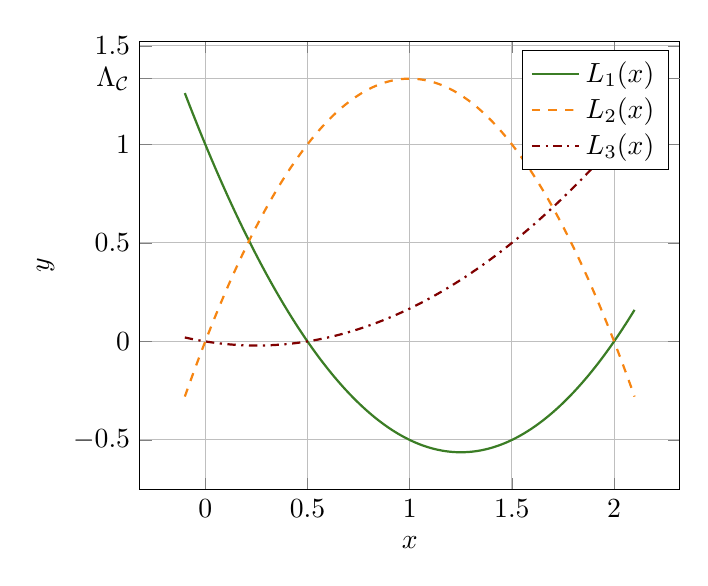
\begin{tikzpicture}
            \begin{axis}[
                extra y ticks={4/3},
                extra y tick labels={$\Lambda_{\mathcal{C}}$},
                xlabel={$x$},
                ylabel={$y$},
                grid,
            ]
                \addplot[domain=-0.1:2.1,samples=200,smooth,thick,color=OliveGreen] {x^2-5*x/2+1};
                \addplot[domain=-0.1:2.1,samples=200,smooth,thick,dashed,color=BurntOrange] {-4*x^2/3+8*x/3};
                \addplot[domain=-0.1:2.1,samples=200,smooth,thick,dashdotted,color=Maroon] {x^2/3-x/6};
                \addlegendentry{$L_1(x)$}
                \addlegendentry{$L_2(x)$}
                \addlegendentry{$L_3(x)$}
            \end{axis}
        \end{tikzpicture}
    \end{center}
\end{frame}

\section{Underdetermined interpolation}

\begin{frame}
    \frametitle{Underdetermined quadratic interpolation}
    
    \begin{block}{}
        To build \alert{one} model, we need~$\mathcal{O}(n^2)$ function evaluations.
        Can we \alert{use less}?
    \end{block}

    \medskip

    Let~$\xpt = \set{y^1, y^2, \dots, y^m}$ be a consistent interpolation set with
    \begin{equation*}
        m \le \frac{1}{2} (n + 1) (n + 2).
    \end{equation*}

    An interpolant~$\objm$ of~$\obj$ on~$\xpt$ is defined by
    \begin{align*}
        \min        & \quad \mathcal{F}(Q)\\
        \text{s.t.} & \quad Q(y^i) = \obj(y^i), ~ i \in \set{1, 2, \dots, m},
    \end{align*}
    where the \alert{functional}~$\mathcal{F}$ reflects a desired \alert{property} or \alert{regularity} of~$\objm$.
\end{frame}

\begin{frame}
    \frametitle{Least Frobenius norm quadratic models}

    The \alert{least Frobenius norm} interpolant~$\objm$ of~$\obj$ on~$\xpt$ is defined by
    \begin{align*}
        \min        & \quad \frac{1}{2} \norm{\nabla^2 Q}_{\mathsf{F}}^2    \\
        \text{s.t.} & \quad Q(y^i) = \obj(y^i), ~ i \in \set{1, 2, \dots, m},
    \end{align*}

    \begin{block}{}
        If~$m \le n + 1$, we have~$B = 0$.
        In practice, we often require that
        \begin{equation*}
            n + 2 \le m \le \frac{1}{2} (n + 1) (n + 2).
        \end{equation*}
    \end{block}

    \medskip

    The notions of \alert{poisedness} and~\alert{$\Lambda$-poisedness} can be directly adapted.
\end{frame}

\begin{frame}
    \frametitle{Least Frobenius norm quadratic models}

    The \alert{KKT conditions} of the variational problem are
    \begin{empheq}[left=\empheqlbrace]{alignat*=1}
        & \sum_{i = 1}^m \lambda_i y^i (y^i)^{\T} = B, \quad \sum_{i = 1}^m \lambda_i = 0, \quad \text{and} \quad \sum_{i = 1}^m \lambda_i y^i = 0,\\
        & c + g^{\T} y^i + \frac{1}{2} (y^i)^{\T} B y^i = \obj(y^i), ~ i \in \set{1, 2, \dots, m}.
    \end{empheq}

    \begin{block}{}
        \begin{enumerate}
            \item This is a \alert{linear system} of~$c$,~$g$, and~$\set{\lambda_1, \lambda_2, \dots, \lambda_m}$.
            \item The matrix~$B$ can be built from~$\set{\lambda_1, \lambda_2, \dots, \lambda_m}$ and~$\xpt$.
            \item Only the \alert{right-hand side} of the linear system depends on~$\obj$.
            \item Instead of storing~$B$, we can store~$\set{\lambda_1, \lambda_2, \dots, \lambda_m}$ and evaluate
            \begin{equation*}
                 B x = \sum_{i = 1}^m \lambda_i \big[ (y^i)^{\T} x \big] y^i \quad \text{and} \quad x^{\T} B x = \sum_{i = 1}^m \lambda_i \big[ (y^i)^{\T} x \big]^2.
            \end{equation*}
        \end{enumerate}
    \end{block}
\end{frame}

\begin{frame}
    \frametitle{Symmetric Broyden update}

    The \alert{least Frobenius norm updating} interpolant~$\objm$ of~$\obj$ on~$\xpt$ is defined by
    \begin{align*}
        \min        & \quad \frac{1}{2} \norm{\nabla^2 Q - B_{\text{old}}}_{\mathsf{F}}^2    \\
        \text{s.t.} & \quad Q(y^i) = \obj(y^i), ~ i \in \set{1, 2, \dots, m},
    \end{align*}
    where~$B_{\text{old}}$ is a \alert{prior estimate} of~$B$.

    \begin{block}{}
        In model-based \alert{DFO methods}, to evaluate~$\objm[k]$, we can set~$B_{\text{old}} = \nabla^2 \objm[k - 1]$.
    \end{block}

    \medskip

    If~$\objm[\text{old}]$ is such that~$\nabla^2 \objm[\text{old}] = B_{\text{old}}$, then~$\objm - \objm[\text{old}]$ solves
    \begin{align*}
        \min        & \quad \frac{1}{2} \norm{\nabla^2 Q}_{\mathsf{F}}^2    \\
        \text{s.t.} & \quad Q(y^i) = \obj(y^i) - \objm[\text{old}](y^i), ~ i \in \set{1, 2, \dots, m}.
    \end{align*}
    These models can then be built as the least Frobenius norm ones.
\end{frame}

\section{An optimal interpolation set}

\begin{frame}
    \frametitle{An important interpolation set}

    \begin{columns}
        \begin{column}{0.55\textwidth}
            Let~$\delta > 0$ be \alert{fixed} and let
            \begin{empheq}[left={z^j = \empheqlbrace}]{alignat*=2}
                & \textcolor{OliveGreen}{0}                 && \quad \text{if~$j = 1$,}\\
                & \textcolor{BurntOrange}{\delta e_{j - 1}} && \quad \text{if~$2 \le j \le n + 1$,}\\
                & \textcolor{Maroon}{-\delta e_{j - n - 1}} && \quad \text{if~$n + 2 \le j \le 2n + 1$.}
            \end{empheq}

            \smallskip

            We consider the interpolation set
            \begin{equation*}
                \mathcal{Z}_m = \set{z^1, z^2, \dots, z^m}.
            \end{equation*}

            \smallskip

            The \alert{smallest~$\ell_p$-ball} containing~$\mathcal{Z}_m$ is
            \begin{equation*}
                \mathcal{B}_p(\delta) = \set{x \in \R^n : \norm{x}_p \le \delta}.
            \end{equation*}
        \end{column}
        \begin{column}{0.45\textwidth}
            \begin{center}
                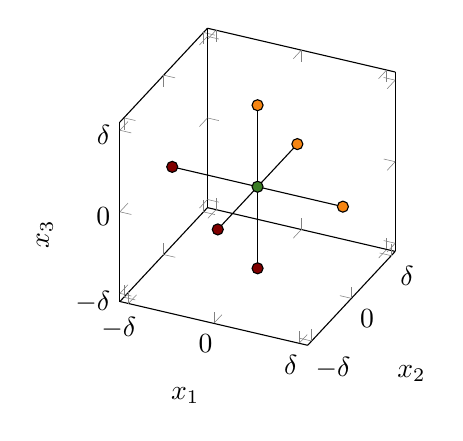
\begin{tikzpicture}
                    \begin{axis}[
                        axis equal image,
                        xmin=-1.1,
                        xmax=1.1,
                        ymin=-1.1,
                        ymax=1.1,
                        zmin=-1.1,
                        zmax=1.1,
                        xtick={-1,0,1},
                        ytick={-1,0,1},
                        ztick={-1,0,1},
                        xticklabels={$-\delta$,$0$,$\delta$},
                        yticklabels={$-\delta$,$0$,$\delta$},
                        zticklabels={$-\delta$,$0$,$\delta$},
                        xlabel={$x_1$},
                        ylabel={$x_2$},
                        zlabel={$x_3$},
                    ]
                        \addplot3[only marks,mark options={fill=OliveGreen}] coordinates{(0, 0, 0)};
                        \addplot3[only marks,mark options={fill=BurntOrange}] coordinates{(1, 0, 0) (0, 1, 0) (0, 0, 1)};
                        \addplot3[only marks,mark options={fill=Maroon}] coordinates{(-1, 0, 0) (0, -1, 0) (0, 0, -1)};
                        \addplot3[no marks] coordinates{(0, 0, 0) (1, 0, 0)};
                        \addplot3[no marks] coordinates{(0, 0, 0) (0, 1, 0)};
                        \addplot3[no marks] coordinates{(0, 0, 0) (0, 0, 1)};
                        \addplot3[no marks] coordinates{(0, 0, 0) (-1, 0, 0)};
                        \addplot3[no marks] coordinates{(0, 0, 0) (0, -1, 0)};
                        \addplot3[no marks] coordinates{(0, 0, 0) (0, 0, -1)};
                    \end{axis}  
                \end{tikzpicture}
            \end{center}
        \end{column}
    \end{columns}
\end{frame}

\begin{frame}
    \frametitle{Explicit formula for the~$\Lambda$-poisedness of~$\mathcal{Z}_m$}

    \begin{block}{}
        For any~$m \ge n + 2$ and~$p \in [1, \infty]$, we have
        \begin{equation*}
            \Lambda_p \eqdef \max_{1 \le i \le m} \max_{x \in \mathcal{B}_p(\delta)} \abs{L_i(x)} = \max_{x \in \mathcal{B}_p(\delta)} \abs{L_1(x)},
        \end{equation*}
        and
        \begin{equation*}
            L_1(x) = 1 - \frac{1}{\delta^2} \sum_{j = 1}^{m - n - 1} x_j^2 - \frac{1}{\delta} \sum_{j = m - n}^n x_j.
        \end{equation*}
    \end{block}

    \begin{columns}
        \begin{column}{0.5\textwidth}
            \begin{center}
                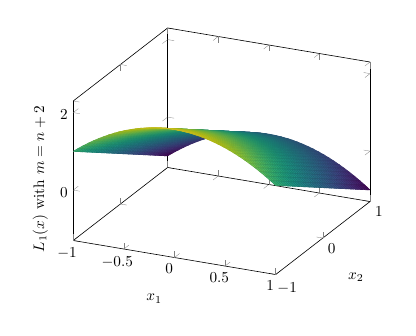
\begin{tikzpicture}[scale=0.55]
                    \begin{axis}[
                        colormap/viridis,
                        xlabel={$x_1$},
                        ylabel={$x_2$},
                        zlabel={$L_1(x)$ with~$m = n + 2$},
                    ]
                        \addplot3[
                            domain=-1:1,
                            domain y=-1:1,
                            samples=40,
                            surf,
                        ]{1-x^2-y};
                    \end{axis}  
                \end{tikzpicture}
            \end{center}
        \end{column}
        \begin{column}{0.5\textwidth}
            \begin{center}
                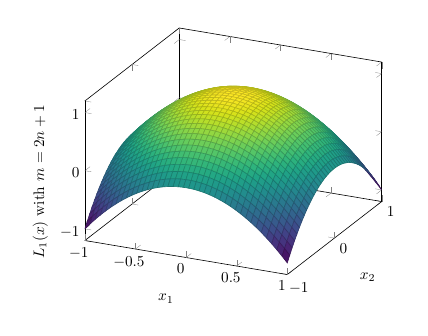
\begin{tikzpicture}[scale=0.55]
                    \begin{axis}[
                        colormap/viridis,
                        xlabel={$x_1$},
                        ylabel={$x_2$},
                        zlabel={$L_1(x)$ with~$m = 2n + 1$},
                    ]
                        \addplot3[
                            domain=-1:1,
                            domain y=-1:1,
                            samples=40,
                            surf,
                        ]{1-x^2-y^2};
                    \end{axis}  
                \end{tikzpicture}
            \end{center}
        \end{column}
    \end{columns}
\end{frame}

\begin{frame}
    \frametitle{Bounds for the~$\Lambda$-poisedness of~$\mathcal{Z}_m$}

    \begin{block}{}
        For any~$m$ and any~$p \in [0, \infty]$, we have
        \begin{equation*}
            1 + (2n + 1 - m)^{\frac{p - 1}{p}} \le \Lambda_p \le n,
        \end{equation*}
        where~$0^0 = 0$ and the lower bound is~$2n + 2 - m$ if~$p = \infty$.
    \end{block}

    \smallskip

    \begin{center}
        \begin{tikzpicture}
            \begin{axis}[
                xtick={22,41},
                xticklabels={$n + 2$,$2n + 1$},
                ytick={1,3,5,7,9},
                xlabel={$m$ (with~$n = 20$)},
                ylabel={Lower bound},
                width=0.9\textwidth,
                height=0.55\textheight,
                samples at={22,...,41},
            ]
                \addplot{ifthenelsefpu((x==41), 1, 2)};
                \addplot{1+(41-x)^(1/2)};
                \addplot{1+(41-x)^(2/3)};
                \addplot{1+(41-x)^(3/4)};
                \addlegendentry{$p = 1$}
                \addlegendentry{$p = 2$}
                \addlegendentry{$p = 3$}
                \addlegendentry{$p = 4$}
            \end{axis}  
        \end{tikzpicture}
    \end{center}
\end{frame}

\begin{frame}
    \frametitle{Some special cases and remarks}

    \begin{block}{}
        For any~$m$, we have
        \begin{empheq}[left={\Lambda_p = \empheqlbrace}]{alignat*=2}
            & 2                             && \quad \text{if~$p = 1$ and~$n + 2 \le m \le 2n$,}\\
            & 1                             && \quad \text{if~$p = 1$ and~$n = 2n + 1$,}\\
            & 1 + \sqrt{2n + 1 - m}         && \quad \text{if~$p = 2$,}\\
            & \max \set{2n + 2 - m, n - 1}  && \quad \text{if~$p = \infty$.}
        \end{empheq}
    \end{block}

    \begin{block}{}
        For any~$p \in [1, \infty]$, if~$m = 2n + 1$, then
        \begin{equation*}
            \Lambda_p = \max \set[\big]{1, n^{\frac{p - 2}{p}} - 1}.
        \end{equation*}
    \end{block}

    \smallskip

    \begin{enumerate}
        \item $\mathcal{Z}_{2n + 1}$ is \alert{optimal} in~$\mathcal{B}_p(\delta)$ for~$p \in [1, 2]$ because~$\Lambda_p = 1$.
        \item $m = 2n + 1$ is optimal for~$\mathcal{Z}_m$ when~$p \in [1, 2]$.
        \item \alert{Conjecture}: $m = 2n + 1$ is optimal for~$\mathcal{Z}_m$ for all~$p \in [0, \infty]$.
    \end{enumerate}
\end{frame}

\section{Conclusion}

\begin{frame}
    \frametitle{Conclusion}
    
    In this talk, we presented
    \begin{enumerate}
        \item basic \alert{concepts of interpolation} and the \alert{Lagrange polynomials};
        \item the notion of~\alert{$\Lambda$-poisedness};
        \item two \alert{underdetermined interpolation} schemes; and
        \item an \alert{optimal interpolation set} used in DFO methods.
    \end{enumerate}

    \bigskip

    In the next talk, we will discuss a new MATLAB/Python package named \alert{PDFO}.
\end{frame}

\appendix

\begin{frame}[t,allowframebreaks]
    \frametitle{References}

	\printbibliography
\end{frame}

\end{document}